\documentclass[russian,english]{scrreprt}

\usepackage{amsmath,amsfonts,amssymb,amsthm,mathtools} % AMS

\usepackage{hyperref}       % hyperref
\hypersetup{				% settings
	unicode=true,           % non-latin letters
	pdftitle={Practical application of the Wilcoxon-Mann-Whitney test in valuation
},   % heading
	pdfauthor={K. A. Murashev},      % Author
	pdfsubject={Wilcoxon-Mann-Whitney test},      % Scope
	pdfcreator={K. A. Murashev}, % Creator
	pdfproducer={K. A. Murashev}, % Producer
	pdfkeywords={Wilcoxon-Mann-Whitney test, U-test} % Keywords
	colorlinks=true,       	% false: links in frames; true: coloured links
	linkcolor=red,          % internal links
	citecolor=green,        % bibliography links
	filecolor=magenta,      % file links
	urlcolor=blue           % URL links
}

\usepackage{url}

\usepackage{babel}

% work with images
\usepackage{graphicx}
\graphicspath{{Images/}}

% work with tables
\usepackage{array, tabularx, tabulary, booktabs, xtab} % additional forms of tables
\usepackage{longtable}  % long tables
\usepackage{multirow} % merge rows

% work with bibliography
\usepackage[backend=biber,bibencoding=utf8,sorting=ynt,maxcitenames=5,sortupper=true,date=iso]{biblatex}

% set the depth of table of contents
\setcounter{tocdepth}{8}

% work with scripts
\usepackage {listings}
\lstloadlanguages{[Latex]Tex, bash, R, Python, SQL}
\lstset{extendedchars=true , % additional symbols
frame=tb, % top & bottom frames
commentstyle=\itshape , % font for comments
stringstyle =\ttfamily % font for 'strings'
keywordstyle=\color{blue} % color for keywords
}

% connecting the automated bibliography package
\usepackage[backend=biber,bibencoding=utf8,sorting=ynt,maxcitenames=5,sortupper=true,date=iso]{biblatex} 

% add sources for bibliography
\addbibresource{/home/kaarlahti/TresoritDrive/Methodics/My/AI_for_valuers/Book/AI_for_valuers_book/Basic_principles.bib}
\addbibresource{/home/kaarlahti/TresoritDrive/Methodics/My/AI_for_valuers/Book/AI_for_valuers_book/LaTeX.bib}
\addbibresource{/home/kaarlahti/TresoritDrive/Methodics/My/AI_for_valuers/Book/AI_for_valuers_book/Mathstat.bib}
\addbibresource{/home/kaarlahti/TresoritDrive/Methodics/My/AI_for_valuers/Book/AI_for_valuers_book/Murashev.bib}
\addbibresource{/home/kaarlahti/TresoritDrive/Methodics/My/AI_for_valuers/Book/AI_for_valuers_book/Python.bib}
\addbibresource{/home/kaarlahti/TresoritDrive/Methodics/My/AI_for_valuers/Book/AI_for_valuers_book/R.bib}
\addbibresource{/home/kaarlahti/TresoritDrive/Methodics/My/AI_for_valuers/Book/AI_for_valuers_book/RussianLaws.bib}
\addbibresource{/home/kaarlahti/TresoritDrive/Methodics/My/AI_for_valuers/Book/AI_for_valuers_book/Sci&Tech.bib}
\addbibresource{/home/kaarlahti/TresoritDrive/Methodics/My/AI_for_valuers/Book/AI_for_valuers_book/Valuation.bib}
\addbibresource{/home/kaarlahti/TresoritDrive/Methodics/My/AI_for_valuers/Book/AI_for_valuers_book/ValuationStandards.bib}
\addbibresource{/home/kaarlahti/TresoritDrive/Methodics/My/AI_for_valuers/Book/AI_for_valuers_book/ZHZL.bib}

\usepackage{bbm} % indicator function

\newcommand{\github}{
	{%
		
\includegraphics[width=3ex,height=3ex,keepaspectratio]{github-seeklogo.pdf}
}
}


% Title Page
\title{Practical application of~the~Wilcoxon-Mann-Whitney test in~valuation.}
\subtitle{Selection of~attributes as~pricing factors based on~the~principle of~unbiased estimates}
\author{\href{https://www.facebook.com/groups/1977067932456703}{K.~A.~Murashev}}

\begin{document}
\maketitle
%
\lstset{language=Python,
	basicstyle=\ttfamily,
	keywordstyle=\color{Blue}\ttfamily,
	stringstyle=\color{Red}\ttfamily,
	commentstyle=\color{Emerald}\ttfamily,
	morecomment=[l][\color{Magenta}]{\#},
	breaklines=true,
	breakindent=0pt,
	breakatwhitespace,
	columns=fullflexible,
	showstringspaces=false
}
%	
\begin{abstract}
	In~their practice appraisers often face the~need to~take into account differences in~quantitative and~qualitative characteristics of~objects. In~particular, one of~the~standard tasks is~to~determine the~attributes that influence the~cost (so-called "pricing factors") and~to~separate them from the~attributes that do~not or~cannot be~determined.
	
	Subjective selection of~attributes taken into account in~determining the~value is~widespread in~valuation practice. In~this case, specific quantitative indicators of~the~impact of~these attributes on~the~cost are~often taken from the~so-called "reference books". While not~denying the~speed and~low cost of~this approach, it~should~be recognized that only data directly observed in~the open markets is~a~reliable basis for~a~value judgment. The priority of~such data over other data, in~particular those obtained by~expert survey, is~enshrined, among others, in~\href{https://www.rics.org/uk/upholding-professional-standards/sector-standards/valuation/red-book/red-book-global/}{RICS Valuation --- Global Standards 2022}~\cite{RVGS-2022}, \href{https://www.rics.org/uk/upholding-professional-standards/sector-standards/valuation/red-book/international-valuation-standards/}{International Valuation Standards 2022}~\cite{IVS-2022}, as~well as~in~\href{http://eifrs.ifrs.org/eifrs/bnstandards/en/IFRS13.pdf}{IFRS~13 "Fair Value Measurement"}~\cite{IFRS-13}. Therefore, we~can say that mathematical methods for~analyzing data from the open market are the~most reliable means of~interpreting market information used in~market research and~predicting the~value of~individual objects.
	
	The aim of~this work is~to~justify the~necessity and~possibility of~using a~rigorous mathematical Wilcoxon--Mann--Whitney test, which allows us~to~answer the~question about the~necessity of~taking into account the~binary attribute as~a~price-generating factor. Instead of~the~judgmental approach, which is~most commonly used by~appraisers in~selecting the~attributes to~be considered in~appraisal, this paper proposes the~idea of~prioritizing the~measuring approach based on~the~results of~a~mathematical test that allows to~draw a~conclusion about the~importance or~otherwise of~the~binary attribute influence on~the~value. It~should~be noted that despite the~fact that the~statistical test under consideration belongs to~frequentist statistics, it, through its~connection to~ROC analysis and~AUC, is~related to~modern machine learning methods, which will~be discussed later in~the~text of~this material. The~presence of~this relationship and~elements of~Bayesian statistics seems particularly interesting and~promising from the~point of~view of~introducing machine learning and~data analysis methods into the~everyday practice of~appraisers.
	
	Users should have some general math background and~basic Python and~R programming skills to~understand and~practice all of~the material in~the~text, but~lack of~that knowledge and~skill is~not~a~barrier to~learning most of~the~material and~implementing the~test in~the~spreadsheet that comes with it.
	
	The material consists of~four blocks:
	\begin{itemize}
		\item a~description of~the~Wilcoxon--Mann--Whitney test (hereafter "U-test"), its probabilistic meaning, and~its relationship to~other mathematical methods;
		\item a~practical implementation of~the~U-test in~a~spreadsheet on~an~example of~test random data;
		\item practical implementation of~the~U-test on~the~real data of~the~residential real estate market of~St.~Petersburg agglomeration by~means of~Python programming language, the~purpose of~the~analysis was~to~check the~significance of~the~difference in~the~unit price between the~objects located in~the~urban and~suburban parts of~the~agglomeration;
		\item practical implementation of~the~U-test on~real data of~residential real estate market of~Almaty by~means of~R programming language, the~purpose of~the~analysis was~to~check the~significance of~difference in~unit price between the~objects sold without demountable improvements and~the~objects sold with them.
	\end{itemize}
	The~current version of~this material, its source code, Python and~R scripts, and~the~spreadsheet are~in~the~repository on~the GitHub portal and~are~available at~the~\href{https://github.com/Kirill-Murashev/AI_for_valuers_book/tree/main/Parts-Chapters/Mann-Whitney-Wilcoxon}{permanent link}~\cite{Murashev:u-test}.
	
	This material and~all of~its~appendices are~distributed under the~terms of~the~\href{https://creativecommons.org/licenses/by-sa/4.0/}{cc-by-sa-4.0} license~\cite{cc-by-sa-4.0}.
\end{abstract}	
%
\tableofcontents
\listoftables
\listoffigures
\lstlistoflistings
%	
\chapter{Technical details}
This material, as~well as~the~appendices to~it, are available at~\href{https://github.com/Kirill-Murashev/AI_for_valuers_book/tree/main/Parts-Chapters/Mann-Whitney-Wilcoxon}{permanent link}~\cite{Murashev:u-test}. The~source code for~this work was~created~using the~language~\href{https://www.ctan.org/}{\TeX}~\cite{TeX:site} with~a~set of~macro extensions~\href{https://www latex-project.org/}{\LaTeXe}~\cite{LaTeX:site}, distribution~\href{https://www.tug.org/texlive/}{TeXLive}~\cite{TeXLive:site} and~Editor~\href{https://www.texstudio.org/}{TeXstudio}~\cite{TeXstudio:site}. The~spreadsheet calculation was~done with \href{https://www.libreoffice.org/discover/calc/}{LibreOffice Calc}~\cite{LO:Calc} (Version: 7.3.4. 2 / LibreOffice Community Build ID: 30(Build:2); CPU threads: 4; OS: Linux 5.11; UI render: default; VCL: kf5 (cairo+xcb) Locale: en-US (en\_US.UTF-8); UI: en-US Ubuntu package version: 1:7.3.4~rc2-0ubuntu0.20.04.1~lo1; Calc: threaded). The~calculation in~\href{https://www.r-project.org/}{R}~\cite{R_language} (version 4.2.1 (2022-06-23) -- "Funny-Looking Kid") was~done~using an~IDE~\href{https://www.rstudio.com/}{RStudio} (RStudio 2022. 02.3+492 "Prairie Trillium" Release (1db809b8, 2022-05-20) for Ubuntu Bionic; Mozilla/5.0 (X11; Linux x86\_64); AppleWebKit/537.36 (KHTML, like Gecko); QtWebEngine/5.12.8; Chrome/69.0.3497.128; Safari/537.36)~\cite{RStudio:official_site}. The~calculation in~\href{https://www.python.org/}{Python}~(Version~3.9.12)~\cite{Python:site} was~performed using the~development environment~\href{https://jupyter.org}{Jupyter Lab} (Version 3.4.2)~\cite{Jupyter:site} and~IDE \href{https://www.spyder-ide.org/}{Spyder} (Spyder version: 5.1.5 None* Python version: 3.9.12 64-bit * Qt version: 5.9.7 * PyQt5 version: 5.9.2
* Operating System: Linux 5.11.0-37-generic)~\cite{Spyder:site}. The~graphics used in~the~subsection \ref{U-test-spreadsheet} were prepared using \href{Geogebra:official-site}{Geogebra}~(Version 6.0.666.0-202109211234)~\cite{Geogebra:official-site}. The~following values were used in~this material as~well as~in~most of~the~works in~the~series:
\begin{itemize}
	\item significance level: $\alpha = 0.05$;
	\item confidence interval: $Pr = 0.95$;
	\item initial position of the pseudo-random number generator: $seed=19190709$.
\end{itemize}
A~dot is~used as~a~decimal point. Most of~the~mathematical notations are~written as~they are~used in~English-speaking circles. For~example, a~tangent is~written as~$\tan$, not~$\tg$. The~results of~statistical tests are~considered significant when
\begin{equation}\label{eq:significance}
p \leq \alpha.
\end{equation}
This decision is~based, in~part, on~the~results of~the~discussion that took place on~\href{researchgate.net}{researchgate.net}~~\cite{RG:p-equals-alpha}.
%
\chapter{Subject of~research}
When working with market data, the~appraiser is~often faced with the~task of~testing the~hypothesis of~whether a~quantitative, ordinal or~nominal attribute has~a~significant effect on~the~price. Real estate market analysts, developers, realtors, employees of~collateral departments of~banks, leasing and~insurance companies, tax inspectors and~other specialists have a~similar task. At~the~same time, it~is~often impossible to~collect large amounts of~data that would allow a~wide range of~machine learning methods to~be~applied. In~some cases appraisers consciously narrow the~area of~data collection to~the~narrow market segment, resulting in~only very small samples of~less than thirty observations at~their disposal. In~this case, the~price data most often has~a~distribution that differs from the~normal one. In~this case, a~rational solution is~to~use U-test. Let~us formulate the~problem:
\begin{itemize}
	\item suppose that we~have two samples of~unit prices for~commercial premises, some of~which have some attribute (e.\,g., having a~separate entrance) and~some of~which do~not;
	\item it~is~necessary to~determine whether the~presence of~this feature has a~significant impact on~the~unit value of~this type of~real estate or~not.
\end{itemize}
At~first glance, according to~established practice, an~appraiser can simply subjectively recognize some attributes as~significant and~others as~not, and~then accept the~adjustment values for~differences in~these attributes from the~reference books. However, as~mentioned above, this approach is~hardly considered best practice because it~lacks any~market analysis. Also, in~that case, it~is~unlikely that such work is~of~any~serious value at~all.

Instead, it~is~possible to~use random samples of~market data and~apply mathematical analysis to~them, allowing scientific and evidence-based conclusions to~be~drawn about the~significance of~a~particular attribute's impact on~value. The~data used in~this paper to~perform the~U-test using Python and~R are~real market data, some of~which were collected by~the author through web scraping and some provided by~colleagues for~the~analysis. The~attached spreadsheet is~set~up so~that test raw data can~be generated in~a~pseudo-random fashion.

The~subject of~this paper is~the~nonparametric Wilcoxon-Mann-Whitney test, specifically designed for~samples that have a~distribution other than normal. This circumstance is~important because the~price data that appraisers deal with most often have this distribution, which excludes the~possibility of~applying the~parametric t-criterion and~z-criterion. In~addition, the~test under consideration is~of~great interest because it~has a~connection to~machine learning methods through AUC, the~calculation of~which through the~formula provided in~the~test framework gives a~value equal to~that calculated by~ROC analysis. Thus, the~study of~the~U-test paves the~way for~a~further dive into the~world of~machine learning, which is~entering many areas of~human activity and~will significantly change the~field of~value estimation in~the~foreseeable future.

The~material contains a~description of~the~test and~instructions for~performing it, sufficient in~the~author's opinion for~its~demonstrable use in~the~estimation process.
%
\chapter{Basic information about the~test}
\section{Assumptions and~formalization of~hypotheses}
First of~all, it~should~be said that, in~spite of~the~stated common name, it~is~more correct to~speak of~two tests:
\begin{itemize}
	\item \href{http://www.machinelearning.ru/wiki/index.php?title=Критерий_Уилкоксона_двухвыборочный}{Wilcoxon rank-sum test} developed by~Frank Wilcoxon in~1945~\cite{MLRU:Wilcoxon-test};
	\item \href{http://www.machinelearning.ru/wiki/index.php?title=Критерий_Уилкоксона-Манна"--~Уитни}{Mann--Whitney~U-test} which is~a~further development of~the~aforementioned criterion developed by~Henry Mann and~Donald Whitney in~1947~\cite{MLRU:Mann-Whitney}.
\end{itemize}
Looking ahead we~can say that the~statistics of~these criteria are~linearly related and~their p-values are~almost the~same which from a~practical point of~view allows us to~talk about variations of~one test rather than two separate tests. This paper uses the~common name throughout the~text, as~well as~a~shortened version of~"U-test" which historically refers to~the~Mann-Whitney test. Some authors\cite{Kobzarq-prikl-mathstat} recommend using the~Wilcoxon rank-sum test when there are~no~assumptions about variance, and the~Mann-Whitney U-test when variance of~the~two samples are~equal. However, the~experimental data indicate that the~Wilcoxon rank-sum test and~Mann-Whitney U-test values are~essentially the~same when the~variance of~the~samples is~significantly different. Adhering to~the~KISS principle~\cite{KISS-principle} underlying the~entire series of~publications, the~author concludes that a~unified approach is~possible. Also remember that the~Wilcoxon signed-rank test is~a~separate test designed to~analyze differences between two matched samples, whereas the~Mann-Whitney U-test discussed in~this paper is~designed to~work with two independent samples.

Suppose that there are~two samples:
\begin{equation*}
x^{m} = (x_{1},x_{2},\ldots,x_{m}), x_{i} \in \mathbb{R};\quad y^{n} = (y_{1},y_{2},\ldots,y_{n}), y_{i} \in \mathbb{R} \quad: m \leq n.
\end{equation*}
%
\begin{itemize}
	\item Both samples are~simple and~random (i.e., \href{https://en.wikipedia.org/wiki/Simple_random_sample}{SRS}~\cite{Wiki:SRS}), the~combined sample is~independent.
	\item The~samples are~taken from unknown continuous distributions \textit{F(x)} and~\textit{G(y)}, respectively.
\end{itemize}
%
\begin{description}
	\item[Simple random sample~(SRS) ---] is~a~subset of~individuals (\emph{a~sample}) chosen from a~larger set (\emph{a~population}) in~which a~subset of~individuals are~chosen randomly, all with the~same probability. It~is~a~process of~selecting a~sample in~a~random way. In~\textbf{SRS}, each subset of~\textit{k}~individuals has~the~same probability of~being chosen for~the~sample as~any~other subset of~\textit{k}~individuals.A~simple random sample is~an~unbiased sampling technique. Equivalent definition: a~sample ${\textstyle x^{m} = (x_{1},x_{2},\ldots,x_{m})}$ is~simple if~the~values~${\textstyle (x_{1},x_{2},\ldots,x_{m})}$ are~realizations of~\textit{m} independent equally distributed random variables. In~other words, the~selection of~observations is~not~only random but also does not~imply any~special selection rules (e.g., choosing every 10th observation).
\end{description}
%
\begin{description}
	\item[The~U-test ---] is~a~nonparametric criterion to~test the~null hypothesis that for~randomly chosen from~two samples of~observations~$x \in X$ and~$y \in Y$ the probability that~\textit{x} is~greater than \textit{y} is~equal to~the~probability that~\textit{y} is~greater than~\textit{x}. In~mathematical language, the~null hypothesis is~written as~follows
	\begin{equation}\label{eq:U-test-null-hypothesis}
	H_{0}:P\{x<y=\frac{1}{2}\}.
	\end{equation}
	For~the~test's own consistency, an~alternative hypothesis is~required, which is~that the~probability that the~value of~a~characteristic of~observation from~\textit{X} is~greater than that of~observation from~\textit{Y} differs upward or~downward from the~probability that the~value of~a~characteristic of~observation from~\textit{Y} is~greater than that of~observation from~\textit{X}. In~mathematical language, the~alternative hypothesis is~written as~follows
	\begin{equation}\label{eq:U-test-alt-hypothesis}
	H_{1}:P\{x<y\} \neq P\{y<x\} \vee P\{x<y\} + 0.5 \cdot P\{x=y\} \neq 0.5.
	\end{equation}
\end{description}
According to~the~basic concept of~the~U-test, if~the~null hypothesis is~true, the~distribution of~the~two samples is~continuous; if~the~alternative hypothesis is~true, the~distribution of~one sample is~stochastically greater than the~distribution of~the~other. In~this case, it~is~possible to~formulate a~number of~null and~alternative hypotheses for~which this test will give a~correct result. His~most extensive generalization lies in~the~following assumptions:
\begin{itemize}
	\item the~observations in~both samples are~independent;
	\item the~data type is~at~least ranked, i.\,e., with respect to~any two observations you can tell which one is~greater;
	\item the~null hypothesis assumes that the~distributions of~the~two samples are equal;
	\item the~alternative hypothesis assumes that the~distributions of~the~two samples are unequal.
\end{itemize}
With a~stricter set of~assumptions than those given above, for~example the~assumption that the~distribution of~the~two samples is~continuous if~the~null hypothesis is~valid and that the~distribution of~the~two samples has a~shift  in~the~distribution if~the~alternative one is~valid i.\,e.~$f_{1}(x)=f_{2}(x+\sigma)$,  we~can say that the~U-test is~a~test for~the~hypothesis of~equality of~medians. In~this case, the~U-test can~be interpreted as~a~test of~whether Hodges--Lehman's estimate of~the~difference in~central tendency measures differs from zero. In~this situation, the~Hodges--Lehman estimate is~the median of~all possible values of~differences between the~observations in~the~first and second samples. However, if~both the~variance and the~shape of~the~distribution of~the~two samples differ, the~U-test cannot correctly test the~medians. Examples can~be shown where the~medians are~numerically equal and the~test rejects the~null hypothesis because of~the~small p-value. Thus, a~more correct interpretation of~the~U-test is~to~use~it to~test the~\href{http://www.machinelearning.ru/wiki/index.php?title=Гипотеза_сдвига}{shift hypothesis}~\cite{MLRU:shift-hypothesis}.
\begin{description}
	\item[Shift hypothesis ---] is~a~statistical hypothesis often considered as~an~alternative to~the~hypothesis of~complete homogeneity of~samples. Let~us have two samples of~data. Let~us also give two random variables~\textit{X} and~\textit{Y}, which are~distributed as~elements of~these samples and have distribution functions~\textit{F(x)} and~\textit{G(y)}, respectively. In~these terms, the~shift hypothesis can~be written as~follows
	\begin{equation}\label{eq:shift-hypothesis}
	H:F(x)=G(x+\sigma)\ : \forall x,\ \sigma \neq 0.
	\end{equation}
\end{description}
In~this case, the~U-criterion is~valid regardless of~the~characteristics of~the~samples.

Simply put, the~essence of~the~U-test is~that it~allows~us to~answer the~question of~whether there~is a~significant difference in~the~value of~the~quantitative attribute of~the~two samples. With regard to~valuation, we~can say that the~use of~this test helps to~answer the~question of~whether it~is~necessary to~take into account one or~another attribute as~a~price-generating factor. It~follows from the~above that by~default we~are talking about a~two-sided test. In~practice, this means that the~test does~not give a~direct answer to~the~question, for~example: "Is~there a~significant excess of~the~unit value of~premises with a~separate entrance to~the~premises that do~not have it. At~the~same time, there~are also one-sided realizations that allow~us to~answer the~question about the~sign of~the~difference in~the~value of~the~attribute in~the~two samples.

In~addition to~the~above requirements for~the~samples themselves, the~conditions for~applying the~U-test are:
\begin{itemize}
	\item the~distribution of~quantitative attribute values of~samples is~different from normal (otherwise it~is advisable to~use parametric Student's t-test or~z-test for~independent samples).
	\item at~least three observations in~each sample, it~is~allowed to~have two observations in~one of~the~samples, provided that there~are at~least five in~the~other sample.
\end{itemize}
To~summarize the~above, there~are three variants of~the~null hypothesis, depending on~the~level of~rigor outlined in~the~table below~\ref{tab:nul-hypothesis-variants}.
\begin{table}[ht]
	\caption{Variants of~the~null hypothesis when using the~U-test in~valuation.}\label{tab:nul-hypothesis-variants}
	\centering
	\begin{tabularx}{\textwidth}{p{0.25\linewidth} p{0.7\linewidth}} 
		\hline
		Type of~hypothesis&Formulation\\
		\hline
		Scientific&The~two samples are~completely homogeneous, i.\,e.~they belong to~the~same distribution, there~is no~shift and the~estimate made for~the~first sample is~unbiased for~the~second one.\\
		\hline
		Practical&The~medians of~the~two samples are~equal to~each other.\\
		\hline
		Set forth in~terms of~valuation&The~difference in~the~attribute between the~two samples of~object-analogues is~not~significant, its accounting is~not required and this attribute is~not a~pricing factor.\\
		\hline
	\end{tabularx}
\end{table}
%
\section{Test implementation}
\subsection{Test statistic}
Suppose that~the elements $x_{1},\ldots,x_{n}$ represent a~simple independent sample from~$X \in \mathbb{R}$, and~the elements $y_{1},\ldots, y_{n}$ represent a~simple independent sample from $Y \in \mathbb{R}$ and the~samples are~independent of~each other. Then the~relevant U-statistic is~defined as~follows:
\begin{equation}\label{eq:U-statistic-base-formula}
\begin{aligned}
U&=\sum_{i=1}^{m} \sum_{j=1}^{n} S (x_{i},y_{j}),\\
&\text{при}\\
S(x,y)&=
\begin{cases}
1,\quad \text{если}\ x>y,\\
\frac{1}{2},\quad \text{если}\ x=y,\\
0,\quad \text{если}\ x<y.
\end{cases}
\end{aligned}
\end{equation}
%
\subsection{Calculation methods}
The~test involves calculating a~statistic usually called the~U-statistic whose distribution is~known if~the~null hypothesis is~true. When working with very small samples, the~distribution is~specified tabularly; when the~sample size is~more than twenty observations, it~is~approximated quite well by~the~normal distribution. There are~two methods of~calculating U-statistics: manual calculation using the~formula \ref{eq:U-statistic-base-formula} or~using a~special algorithm. The~first method, due~to its~labor-intensive nature, is~only suitable for~very small samples. The~second method can~be formalized as~a~step-by-step set of~instructions and will~be described below.
\begin{enumerate}
	\item You must construct a~common variation series for~the~two samples and then assign a~rank to~each observation, starting with one for~the~smallest of~them. If~there are~ties, i.\,e. groups of~repeating values (such a~group can~be, e.\,g., only two equal values), each observation from such a~group is~assigned a~value equal to~the~median of~the~group ranks before adjustment (for example, in~the~case of~a~variation series (\textit{3, 5, 5, 5, 5, 8}) the~ranks before adjustment are~(\textit{1, 2, 3, 4, 5, 6}) after --- (\textit{1, 3.5, 3.5, 3.5, 3.5, 6}).
	\item It~is necessary to~calculate the~sums of~the~ranks of~the~observations of~each sample, denoted as~${R_{1},\ R_{2}}$ respectively. In~this case, the~total sum of~ranks can~be calculated by~the~formula
	\begin{equation}\label{eq:common-R}
	R = \frac{N(N+1)}{2},
	\end{equation}
	where~\textit{N} ---the~total number of~observations in~both samples.
	%
	\item Next, we~calculate the~U-value for~the~first sample:
	\begin{equation}\label{eq:U1}
	U_{1}=R_{1}-\frac{n_{1}(n_{1}+1)}{2},
	\end{equation}
	where $R_{1}$ ---the~sum of~ranks of~the~first sample, $n_{1}$ --- the~number of~observations in~the~first sample.
	%
	\item The~U-value for~the~second sample is~calculated in~the~same way:
	\begin{equation}\label{eq:U2}
	U_{2}=R_{2}-\frac{n_{2}(n_{2}+1)}{2},
	\end{equation}
	where $R_{2}$ ---the~sum of~ranks of~the~second sample, $n_{2}$ --- the~number of~observations in~the~second sample.
	
	From the~above formulas it~follows that
	\begin{equation}\label{eq:U1-U2-relation}
	U_{1}+U_{2} = R_{1}-\frac{n_{1}(n_{1}+1)}{2} + R_{2}-\frac{n_{2}(n_{2}+1)}{2}.
	\end{equation}
	It~is~also known that
	\begin{equation}\label{eq:R-N-relation}
	\begin{cases}
	R_{1}+R_{2}=\dfrac{N(N+1)}{2}\\
	N=n_{1}+n_{2}.
	\end{cases}
	\end{equation}
	Then
	\begin{equation}\label{eq:check-U-value}
	U_{1}+U_{2}=n_{1}n{2}.
	\end{equation}
	Using this formula as~a~control ratio can~be useful for~checking the~correctness of~calculations in~a~spreadsheet processor.
	%
	\item From the~two values of~$U_{1},\ U_{2}$ in~all cases we~choose the~smaller which will~be the~U-statistic and~used in~further calculations. Let~us denote it~as~\emph{U}.
\end{enumerate}
%
\subsection{Interpretation of~the~result}
For~a~correct interpretation of~the~test result it~is necessary to~specify:
\begin{itemize}
	\item size of each sample;
	\item values of~the~measure of~central tendency for~each sample (given the~nonparametric nature of~the~test, the~median appears to~be the~appropriate measure of~central tendency);
	\item the~value of~the~U-statistic itself;
	\item the~\href{https://en.wikipedia.org/wiki/Effect_size#Common_language_effect_size}{CLES} index~\cite{Wiki:CLES} the~value of~which is~equivalent to~the~AUC and~$\rho$-statistic;
	\item \href{https://en.wikipedia.org/wiki/Effect_size#Rank-biserial_correlation}{rank-biserial correlation coefficient~(RBC)}~\cite{Wiki:rank-biserial-correlation};
	\item the~accepted level of~significance (usually 0.05);
	\item the~calculated p-value.
\end{itemize}
The~concept of~U-statistic was discussed earlier and most of~the~other indicators are widely known and do~not require any particular consideration. 
\subsubsection{CLES = $\rho$-statistic = AUC}
First of~all, it~must~be said that all of~these indicators are~equivalent to~each other. Thus
\begin{equation}\label{eq:AUC=CLES}
CLES = f = AUC_{1} = \rho.
\end{equation}
\paragraph{Common language effect size~(CLES)}
\begin{description}
	\item[Common language effect size~(CLES) ---] is the~probability that the~value of~a~randomly chosen observation from the first sample is greater than the~value of~a~randomly chosen observation from the second sample. This indicator is~calculated by~the~formula
	\begin{equation}\label{eq:CLES}
	CLES = \frac{U_{1}}{n_{1}n_{2}}.
	\end{equation}
	The designation \emph{f~(favorable)} is~often used instead of~\emph{CLES}. This sample value is~an~unbiased estimate of~the~value for~the~entire population of~objects belonging to~the~set.	
\end{description}
It~should~be noted that the~value and meaning of~this indicator is~equivalent to~the~value and meaning of~the ~\href{https://en.wikipedia.org/wiki/Receiver_operating_characteristic}{AUC}\cite{Wiki:ROC}. Thus, we~can say that this indicator characterizes the~quality of~ the~U-test as~a~binary classifier.
\begin{equation}\label{eq:AUC}
CLES = f = AUC_{1} = \frac{U_{1}}{n_{1}n_{2}}.
\end{equation}
The~relationship between the~U-statistic and~AUC is~discussed in~\ref{U-AUC}.
%
\paragraph{$\rho$-statistic}
A~statistic called~$\rho$ that is~linearly related to~U and widely used in~studies of~categorization (discrimination learning involving concepts), and elsewhere, is~calculated by~dividing~U by~its maximum value for~the~given sample sizes, which is~simply $n1 \times n2$. Thus, $\rho$ is~a~non-parametric measure of~the overlap between two~distributions; it~can take values between 0 and~1, and it~is~an~estimate of~$P(Y > X) + 0.5 P(Y = X)$, where \textit{X} and~\textit{Y} are~randomly chosen observations from the~two distributions. Both extreme values represent complete separation of~the~distributions, while a~$ρ = 0.5$ represents complete overlap. This statistic is~useful in~particular when despite a~large p-value the~medians of~the~two samples are~essentially equal to~each other. 
%
\subsubsection{Rank-biserial correlation~(RBC)}
The method of~representing the~measure of~impact for~the~U-test is~to~use a~measure of~rank correlation known as~rank-biserial correlation~(hereafter RBC). As~in~the~case of~other measures of~correlation, the~value of~the~RBC coefficient has a~range of~values [-1;1], with a~zero value indicating the~absence of~any relationship. The~RBC coefficient is~usually denoted as~\textit{r}. A~simple formula based on~the~CLES~(AUC, t, $\rho$) value is~used to~calculate it. Let~us state the~hypothesis that in~a~pair of~random observations, one of~which is~taken from the~first sample and the~other from the~second, the~value of~the~first is~greater.Let's write it~down in~mathematical language:
\begin{equation}\label{eq:RBC-hypothesis}
H: x_{i} > y_{j}, \quad x \ \in X,\ y \in Y.
\end{equation}
Then the~value of~the~RBC coefficient is~the~difference between the~proportion of~random pairs of~observations that are~favorable~(f) to~the~hypothesis and the~complementary proportion of~random pairs that are unfavorable to~the~hypothesis. Thus, this formula is~a~formula for~the~difference between the~CLES scores for~each of~the~groups.
\begin{equation}\label{eq:RBC-formula-1}
r = f - u = CLES_{1} - CLES_{2} = f - (1 - f)
\end{equation}
There are also a~number of~alternative formulas that give identical results:
\begin{equation}\label{eq:RBC-formula-2}
r = 2f -1 = \frac{2U_{1}}{n_{1}n_{2}}-1 = 1 - \frac{2U_{2}}{n_{1}n_{2}}.
\end{equation}
%
\subsection{Calculation of~the~p-value and the~final test of~the~null hypothesis}
If~the~number of~observations in~both samples is~large enough, the~U-statistic has~an~approximately normal distribution. Then its~\href{https://en.wikipedia.org/wiki/Standard_score}{standardized value}~(z-score)~\cite{Wiki:z-score} can~be calculated by~the formula
\begin{equation}\label{eq:z-score}
z = \frac{U-m_{U}}{\sigma_{U}},
\end{equation}
where~$m_{U}$ is~mean for~\textit{U} and $\sigma_{U}$ is~its~standard deviation. A~visualization of~the~concept of~\emph{standardized value for~a~normal distribution} is~shown in~Figure~\ref{fig:z-score}.
%
\begin{figure}[ht]
	\centering
	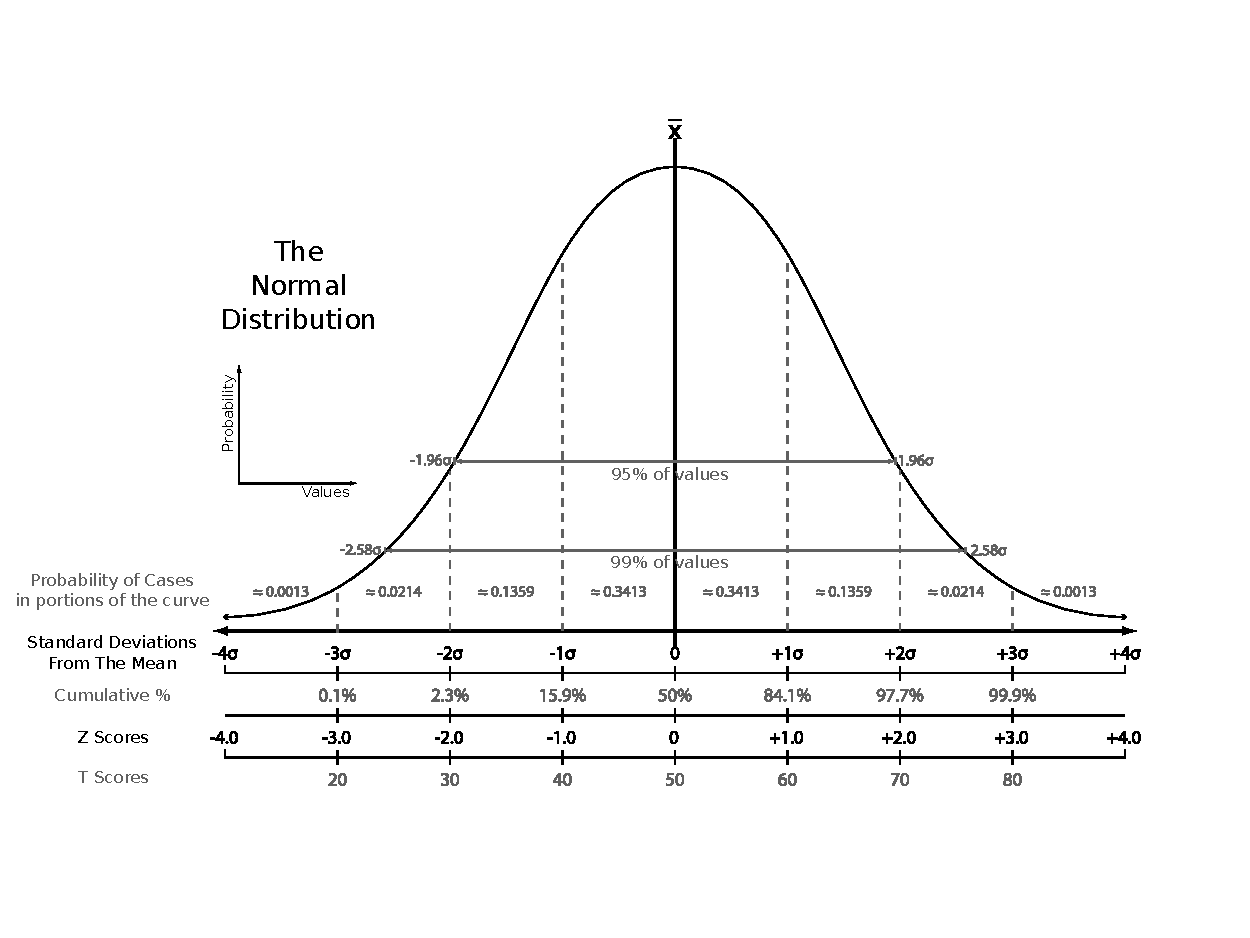
\includegraphics[width=0.8\textwidth]{The_Normal_Distribution.pdf}
	\caption{A~visualization of~the~concept of~standardized value for~a~normal distribution \cite{Wiki:z-score}}\label{fig:z-score}
\end{figure}
%
The mean for~the~U is~calculated by~the~formula
\begin{equation}\label{eq:U-mean}
m_{U} = \frac{n_{1}n_{2}}{2}.
\end{equation}
The~formula for~the standard deviation in~the case of~no~ties is~as~follows:
\begin{equation}\label{eq:standard-deviation-no-ties}
\sigma_{U} =  \sqrt{\frac{n_{1}n_{2}(n_{1}+n_{2}+1)}{12}}.
\end{equation}
In~case of~the~presence of~tied ranks, a~different formula is~used:
\begin{equation}\label{eq:standard-deviation-ties}
\sigma_{U_{ties}} = \sqrt{\frac{n_{1}n_{2}(n_{1}+n_{2}+1)}{12} - \frac{n_{1}n_{2}\sum_{k=1}^{K}({t_{k}}^{3} - t_{k})}{12n(n-1)}} = \sqrt{\frac{n_{1}n_{2}}{12} \left((n+1)-\frac{\sum_{k=1}^{K}({t_{k}}^{3} - t_{k})}{n(n-1)}\right)},
\end{equation}
where~$t_{k}$ is~the~number of~observations with rank~\textit{k} and \textit{K} is~the~total number of~tied ranks. Then, by~obtaining a~standardized value~(z-score) and~using an~approximation of~the~standard normal distribution, the~p-value for~a~given level of~significance (usually~0.05) is~calculated. The~interpretation of~the~result is~as~follows:
\begin{equation}\label{eq:p-interpretation}
\begin{aligned}
p &\leq 0.05 \Rightarrow \text{the~null hypothesis is~rejected}\\
p &> 0.05 \Rightarrow \text{the~null hypothesis can~not~be rejected}.
\end{aligned}
\end{equation}
However, there is~also an~alternative interpretation:
\begin{equation}\label{eq:p-interpretation-2}
\begin{aligned}
p &< 0.05 \Rightarrow \text{the~null hypothesis is~rejected}\\
p &\geq 0.05 \Rightarrow \text{the~null hypothesis can~not~be rejected}.
\end{aligned}
\end{equation}
To~date, there is~no~unambiguous position on~how the~situation when $p = \alpha$ should~be interpreted. This paper uses the~version described in~\ref{eq:p-interpretation}.
%
\section{Relationship to~other statistical tests}
\subsection{Comparison of~Wilcoxon-Mann-Whitney U-test with Student's t-test}
You often hear that the~U-test is~the~nonparametric counterpart of~the~Student's t-test, designed for~data whose distribution differs from the~normal one. From a~purely practical point of~view, we~can indeed say that in~the~case of~a~normal distribution it~is~advisable to~determine whether there is~a~significant difference between the~two samples by~means of~the~t-test, and in~the~case of~a~distribution that differs from the~normal by~means of~the~U-test. Thus, it~can~be said that these tests are~used for~the~same ultimate purpose.

However, the~mathematical meaning of~the~U-test and~the~t-test are~significantly different. As~stated earlier, the~U-test is~designed to~test the~null hypothesis, which is~that for~randomly chosen from two samples of~observations $x \in X$ and~$y \in Y$ the~probability that~\textit{x} is~greater than~\textit{y} is~equal to~the~probability that~\textit{y} is~greater than~\textit{x}, the~alternative hypothesis carries the~claim that these probabilities are~not equal. At~the~same time, the~t-test is~designed to~test the~null hypothesis that the~means of~the~two samples are~equal, while the~alternative hypothesis is~that the~means of~the~two samples are~not~equal. In~this regard, when comparing these tests, we~should keep in~mind that, in~general, the~U-test and~the~t-test check different null hypotheses, although they have partly similar practical meaning. The~result of~the~U-test is~most often very close to~the~result of~the~two-sample t-test for~ranked data. Table~\ref{tab:U-test-t-test-comparison} then provides a~general comparison of~the~U-test with the~t-test.
%
\begin{table}[ht]
	\caption{Properties of~the~U-test relative to~the~t-test.}  \label{tab:U-test-t-test-comparison}
	\centering
	\begin{tabularx}{\textwidth}{p{0.15\linewidth} p{0.8\linewidth}} 
		\hline
		Property&Description\\
		\hline
		Applicability to~ordinal data&When working with ordinal~(rank) data, rather than quantitative data, the~U-test is~preferable to~the~t-test, remembering that the~distance between neighboring values of~the~variation series cannot~be considered constant.\\
		\hline
		Robustness&Since the~U-test handles the~sum of~ranks rather than trait values, it~is less likely than the~t-test to~erroneously indicate significance due~to outliers. However, in~general, the~U-test is~more prone to~type~I error in~the~case when the~data simultaneously have the~property of~heteroscedasticity and~have a~distribution other than normal.\\
		\hline
		Efficiency&In~the~case of~a~normal distribution, the~asymptotic efficiency of~the~U-test is~$\frac{3}{4}\pi \approx 0.95$ of~the~t-test~\cite{U-test-efficiency}. If~the~distribution differs significantly from the~normal one and~the~number of~observations is~large enough, the~efficiency of~the~U-test is~significantly higher than the~efficiency of~the~t-test~\cite{Practical-Nonparametric-Statistics}. However, this efficiency comparison should~be interpreted with caution, because the~U-test and the~t-test examine different hypotheses and~estimate different values. In~the~case, for~example, of~the~need to~compare means, the~use of~the~U-test is~not justified in~principle.\\
		\hline
	\end{tabularx}
\end{table}
%
\subsection{Alternative tests in~the~case of~inequality of~distributions}
If~it~is necessary to~test the~stochastic ordering of~two samples (i.e.~the~alternative hypothesis: $H1:\ P(Y>X)+0.5P(Y=X)\neq0.5$) without assuming equality of~their distributions (i.e.~when the null hypothesis is~$H0:\ P(Y>X)+0.5P(Y=X)=0.5$ but not $F(X)=G(Y)$), more appropriate tests should~be used. These include the~Brunner-Munzel test~\cite{Bruner-Munzel-test-1}, which is~a~heteroskedasticity-resistant analog of~the~U-test, and the~Fligner-Policello test~\cite{Fligner-Policello-test}, which is~a~test for~equality of~medians. In~particular, in~the~case of~a~more general null hypothesis $H0:\ P(Y>X)+0.5P(Y=X)=0.5$, the~U-test can often lead to~a~type~I error even in~the case of~large samples (especially in~the~case of~disparity of~variance and significantly different sample sizes), so~that in~such cases the use of~alternative tests is~preferable~\cite{U-test-vs-Bruner-Munzel-test}. Thus, in~the absence of~the assumption of~equality of~distributions in~case the null hypothesis is~valid, the use of~alternative tests will~be preferable.
%
\clearpage 

\nocite{Essential-Statistical-Inference}
\nocite{AUC-optimization}
\nocite{Mann-Whitney-1947}
\nocite{Optimizing-classifier-performance}
\nocite{ROC-R-1}
\nocite{ROC-AUC-1}
\nocite{ROC-AUC-meets-U-R-1}

\printbibliography
\end{document}          
